\begin{frame}\begin{center}
		\LARGE\textbf{Asymptotic distribution}
\end{center}\end{frame}
%-------------------------------------------------------------------------------
%-------------------------------------------------------------------------------
\begin{frame}\textbf{Asymptotic distribution}\vspace{0.3cm}

Under some regularity conditions, the GMM estimator has the following asymptotic distribution.

\begin{align*}
\sqrt{n}(\hat{\beta} - \beta_0) \xrightarrow{d} \N (0, V),
\end{align*}
where $V = (G^\prime A G)^{-1} G^\prime A \Omega A G (G^\prime A G)^{-1}$ with $G = E[\partial g_i(\beta_0) / \partial \beta]$ and $\Omega = E[g_i(\beta_0)g_i(\beta_0)^\prime]$.\\\vspace{0.3cm}

$\Rightarrow$ asymptotic variance depends on the choice of the weighing matrix $A$

\end{frame}
%-------------------------------------------------------------------------------
%-------------------------------------------------------------------------------
\begin{frame}

The optimal weighing matrix $A = \Omega^{-1}$ the asymptotic variance simplifies to

\begin{align*}
V = (G^\prime  \Omega^{-1} G)^{-1}\\
\end{align*}

What makes a good moment?\vspace{0.3cm}
\begin{itemize}\setlength\itemsep{1em}
\item small $\Omega$, small sample variation of the moment
\item large $G$, moment informative on true value
\end{itemize}


\end{frame}
%-------------------------------------------------------------------------------
%-------------------------------------------------------------------------------
\begin{frame}

\begin{figure}[htp]\centering
\caption{Weak identification}
\scalebox{0.70}{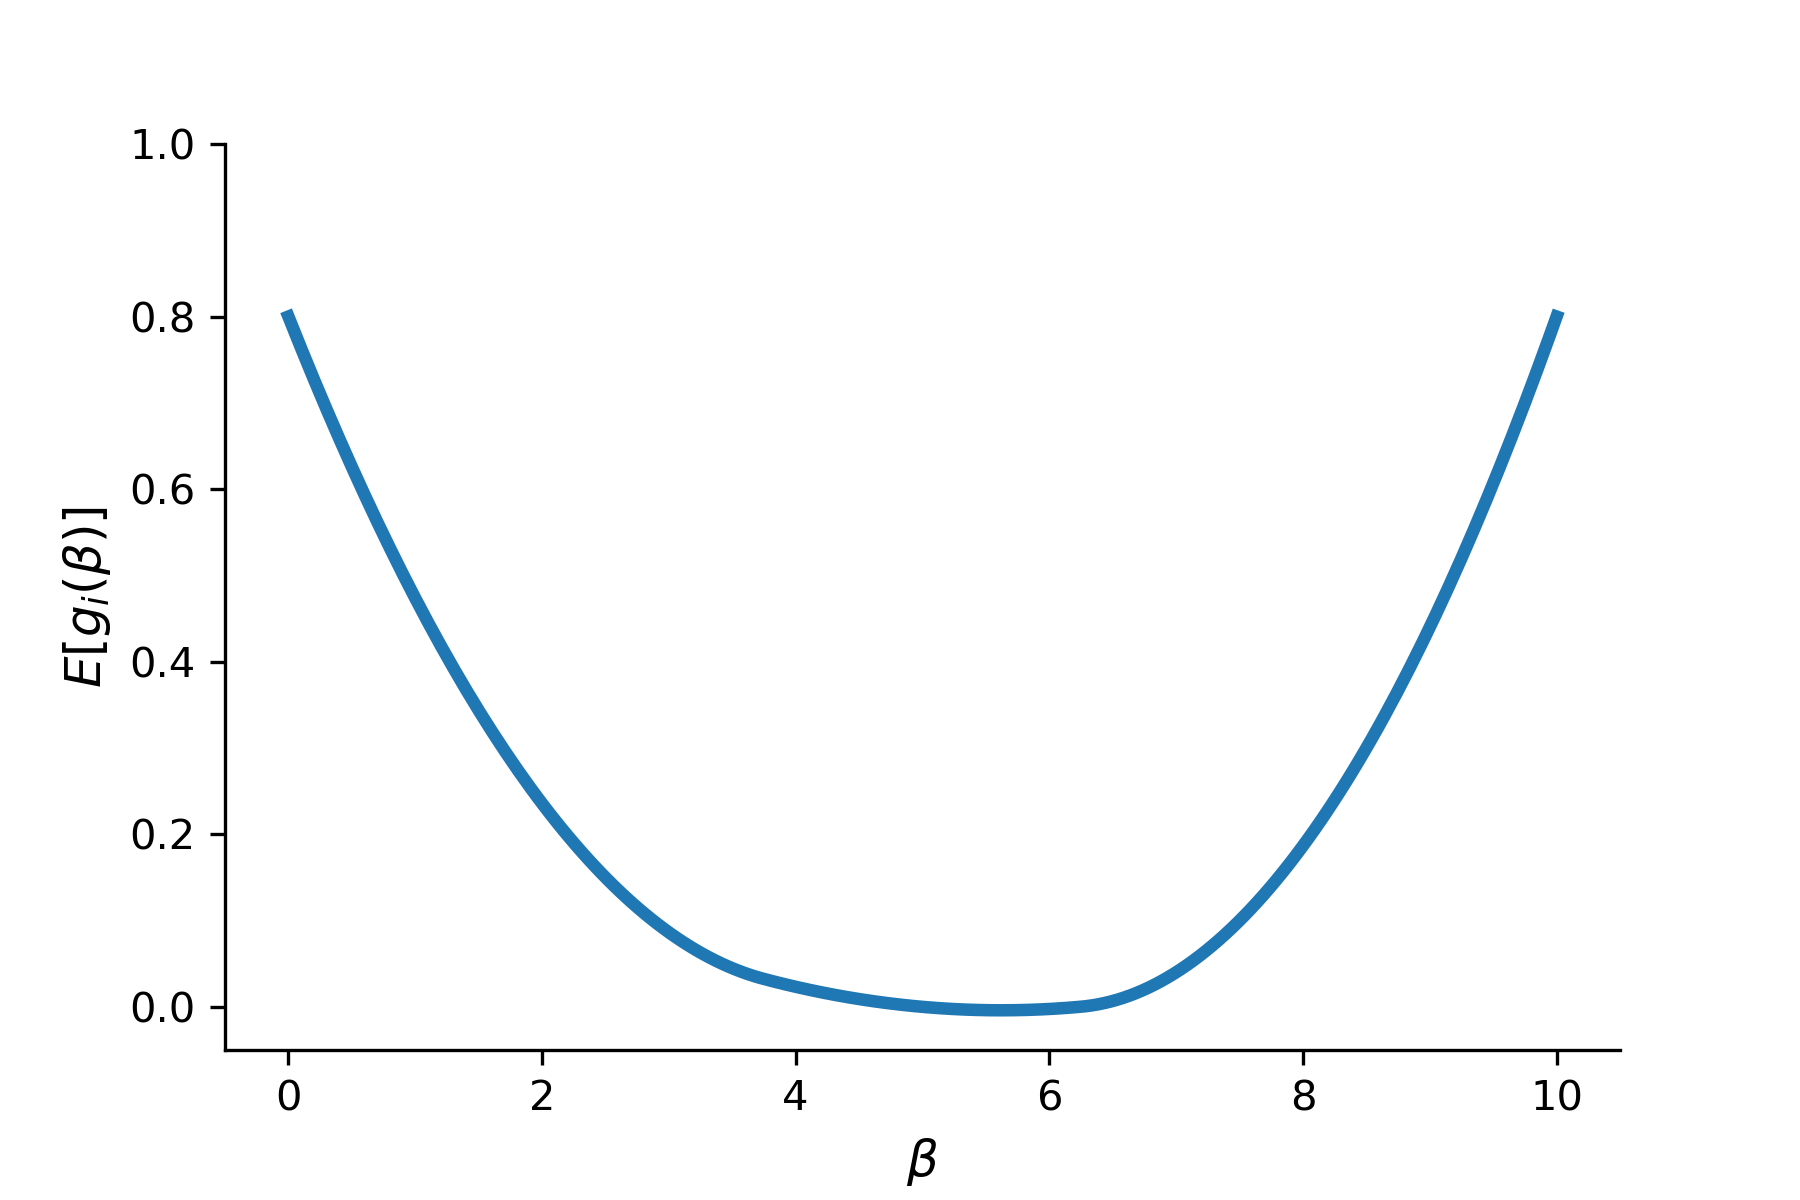
\includegraphics{material/weak-identification}}
\end{figure}
\end{frame}
%-------------------------------------------------------------------------------
%-------------------------------------------------------------------------------
\begin{frame}
\begin{figure}[htp]\centering
\caption{Sharp identification}
\scalebox{0.70}{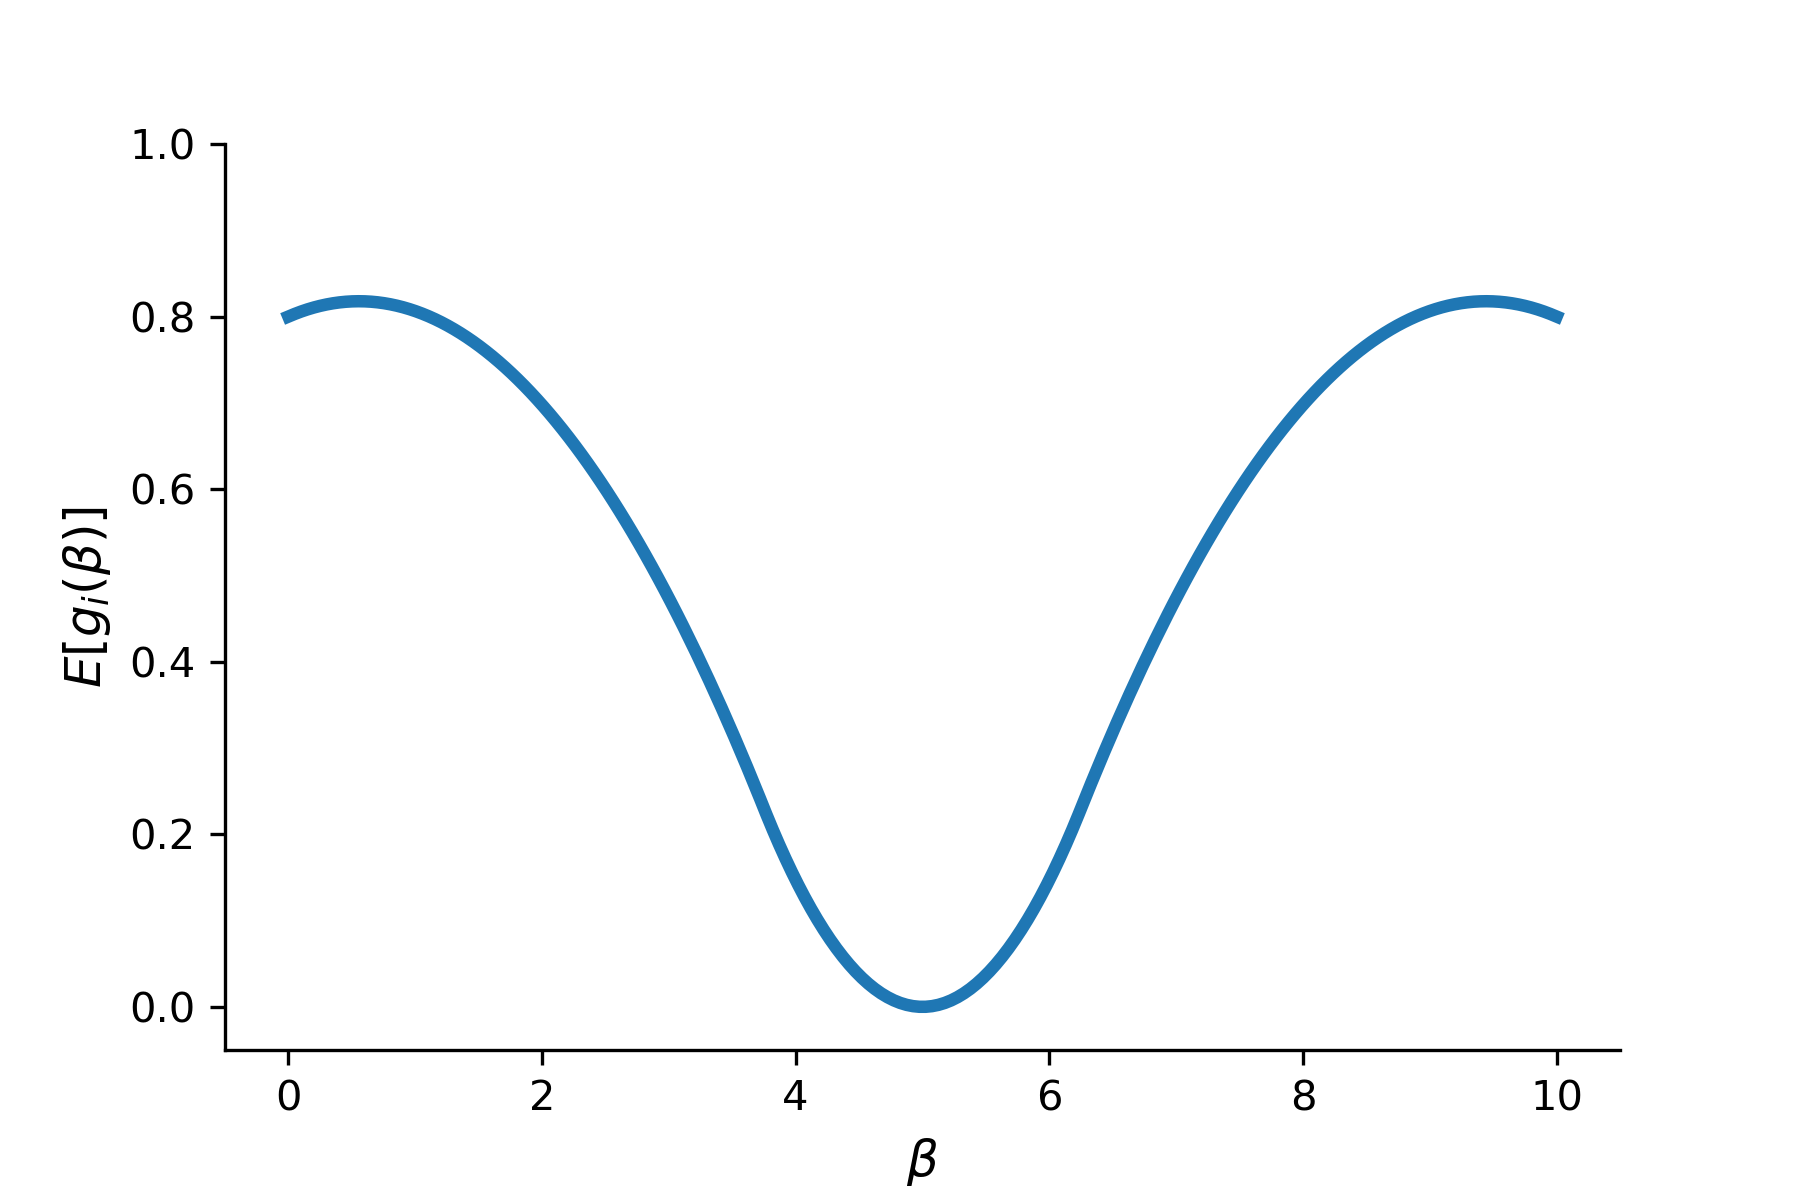
\includegraphics{material/sharp-identification}}
\end{figure}
\end{frame}
%-------------------------------------------------------------------------------
%-------------------------------------------------------------------------------
\begin{frame}\textbf{Instrumental variables}\vspace{1cm}

\begin{center}
Let's continue our example on the blackboard.
\end{center}

\end{frame}
%-------------------------------------------------------------------------------
%-------------------------------------------------------------------------------
